Robotic system design is a mandatory course on the 3rd semester in the robotic systems master program. The course contains 6 student groups, where each has been selected to work with either a mobile robot or workcell robot. This group 3 is working with the workcell robot, i.e PA10 or Staubli robot. The project goals is to create a solution among all the groups to manufacture a multi robot production facility that handles LEGO-bricks orders. The worokcell robots will sort the LEGO-bricks and the mobile robots will handle transportation. A LEGO-dispenser will be available in the project, which will provide the system with LEGO-bricks. The scene will take place in the RoboLab at the university. 
\\
\\
The scene in Robolab has been illustrated, with reference to the course description, in figure \ref{fig:workZone}. Here there will be 3 mobile robots and 3 workcell robots working together to perform the project goal. 


\begin{figure}[ht]
\centering
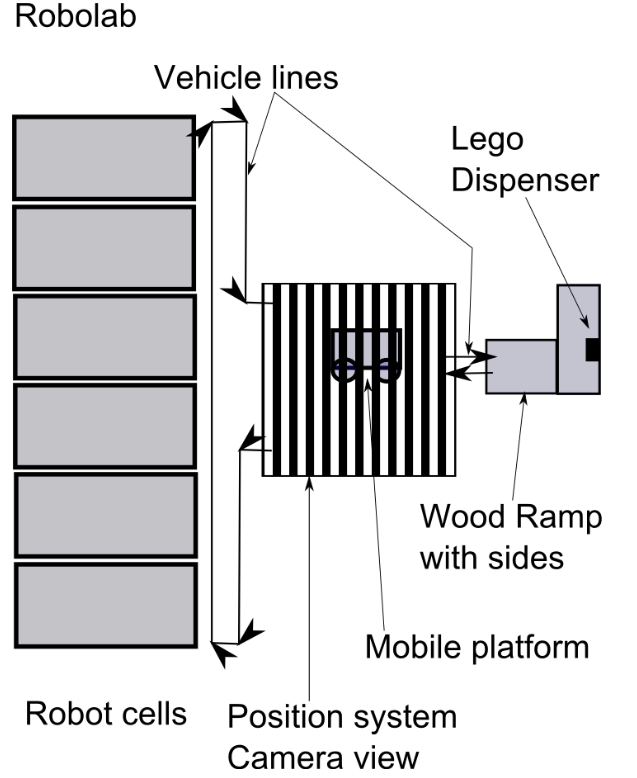
\includegraphics[scale=0.4]{images/workZone.png}
\caption{Setup of the multi robot production facility, where workcell robots sorting LEGO bricks in robot cells and mobile robots transport the LEGO-brick in Robolab}
\label{fig:workZone}
\end{figure}

\section{Project setup}
A general block diagram was created to start identifying different components for the system in the robot cell. This is illustrated in figure \ref{fig:hardwarediagram}. 

In overall the system for the robot cell contains the following components
\begin{itemize}
\item{PA10 or Staubli workcell robot}
\item{Conveyor belt}
\item{Carmine RGB-D sensor}
\item{PLC}
\item{Motor controller for the conveyor belt}
\item{Protocol interface to MES server}
\end{itemize}

\begin{figure}[ht]
\centering
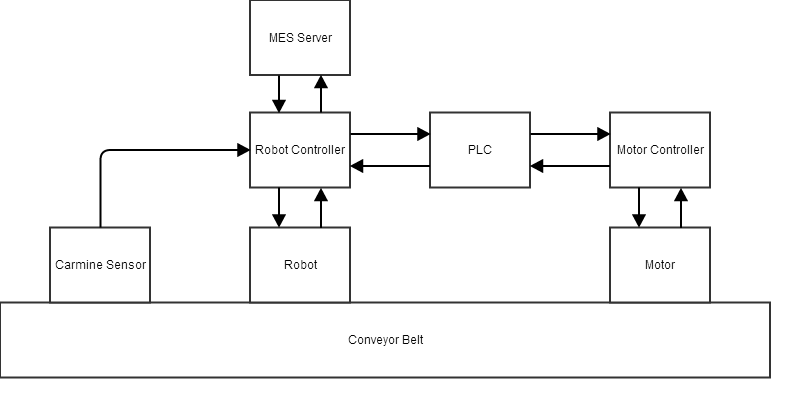
\includegraphics[width=\textwidth]{images/hardwarediagram.png}
\caption{Generel blockdiagram of the different component for the system of the workcell robot in the robot cell}
\label{fig:hardwarediagram}
\end{figure}

%\section{Project description}
%Initially the workcell robot is standing in a initial configuration and the system in the robot cell is waiting for status request or order request from the MES server. If an order is placed in the MES system, an mobile robot will be ordered to pick up bricks from the LEGO dispenser, which feed the mobile robot with a random number of LEGO bricks in a random shape and color. However limitations on the LEGO-bricks will be stated later in the project. 
%
%The MES server will be sending status request for all the robot workcell and receive status if workcells are available or not.
%While the mobile robot has been received LEGO-bricks from the dispenser, the MES server has arranged which workcell the current mobile robot has to go to. After the mobile robot acknowledge this order, MES server is sending status report to system in workcell. While mobile robot is under way, the system in workcell gets ready for incomming load-off. The moment the mobile robot get to the barcode, that indicate the target workcell, the mobile robot will send status to the MES server. The MES server will then send loading request to the given workcell, in order begin the loading and sorting of LEGO-bricks.  The workcell system will send status report back to MES server to indicate that the system is in process of sorting. The MES sever are able to send the mobile robot back to initial waiting position in the local GPS zone. Doing the sorting procedure, all the LEGO bricks will be places in either a order box or spare-part box. When the system in the workcell is done sorting LEGO bricks, the status of boxes is send back to the MES server. If the order is not finish, collecting LEGO bricks procedure will be executed. If the order is finish, collecting orders procedure will be executed, i.e mobile robot will be ordered to go to the current workcell and pick up the order box. If the spare-part box are reaching its maximum capacity, the MES server will be informed, which creates an order procedure. 